% 
% Literatuurstudie
% @author Pieter Maene <pieter.maene@student.kuleuven.be>
%

\chapter{Literatuurstudie}
\label{chap:literatuurstudie}

Deze thesis handelt over methoden voor online verkiezingen. Een interessant verwant probleem zijn systemen die gebruik maken van papier. In dit hoofdstuk wordt specifiek gekeken naar papieren voter-verifiable systemen.

\npar In \ref{sec:ls:geschiedenis} wordt eerst een kort overzicht van de geschiedenis van stemsystemen gegeven. Vervolgens worden de voornaamste vereisten bekeken waaraan deze systemen moeten voldoen (\ref{sec:ls:vereisten}). Belangrijk hierbij is de definitie van een voter-verifiable systeem. Tot slot worden zowel systemen onderzocht die geen gebruik maken van cryptografische methoden (\ref{sec:ls:systemen_zonder_cryptografie}) als deze die daar wel op steunen (\ref{sec:ls:systemen_met_cryptografie}).

\section[Geschiedenis]{Geschiedenis~\cite{adida_advances_in_cryptographic_voting_systems}}
\label{sec:ls:geschiedenis}

Onze samenleving heeft een rijke geschiedenis van stemprocedures, die teruggaat tot Athene in het oude Griekenland. Hier bracht men een negatieve stem uit op een potscherf. In deze paragraaf bekijken we kort enkele methodes die bepalend zijn geweest voor de manier waarop we vandaag werken.\cite{wiki:ostracon}

\npar Sinds de uitvinding van het geheime stembiljet in 1858 in Australi\"e, is er eigenlijk niet meer zoveel veranderd. In dit systeem worden de biljetten op voorhand gedrukt door de staat en veilig bewaard tot op de stemdag. Elke stemgerechtigde krijgt op de stemdag een biljet waarna hij zijn stem uitbrengt in een stemhokje. Het grootste voordeel van deze methode ligt in het feit dat elke stem geheim is.

\npar Deze stemmethode maakte het daarnaast ook mogelijk om mechanische (en later elektrische) machines te gebruiken. Mechanische systemen werden gebruikt in grotere gemeenschappen en waren gebaseerd op hendels en mechanische tellers. De eerste van deze machines werd in 1892 ingevoerd in New York. Rond 1960 werden de eerste elektrische machines ingevoerd. Deze maakten gebruiken van optische scans. Bij deze systemen moest de stem meestal op een specifieke manier aangegeven worden, bijvoorbeeld door het inkleuren van bolletjes.

\npar Sinds 2000 worden steeds vaker DRE machines gebruikt. Hierop draait speciale stemsoftware die de keuze van de kiezer digitaal vastlegt. Deze machines maken het stemproces aanzienlijk eenvoudiger. Het grootste probleem is dat de kiezer geen enkele bevestiging krijgt en dat hij deze machines dus volledig moet vertrouwen.\cite{wiki:dre_voting_machine}

\npar Het gebrek aan controle door de kiezer bij DRE vormde de aanleiding voor het ontwerpen van VVPAT machines. Hierbij toont de machine de kiezer een afgeschermde afdruk van zijn stem, waarna hij deze kan accepteren of weigeren. Op die manier kan de kiezer verifi\"eren of zijn stem correct is. In principe zouden bij een hertelling dan ook deze papieren tickets en niet de digitale data gebruikt moeten worden.\cite{wiki:vvpat}

\section{Vereisten}
\label{sec:ls:vereisten}

Bij het ontwerpen van een stemsysteem zijn er twee tegenstrijdige doelen. Enerzijds moet het mogelijk zijn dat de kiezer thuis kan controleren of zijn stem juist meegeteld is. Anderzijds mag diezelfde persoon niet kunnen bewijzen voor wie hij precies gestemd heeft, noch mag het mogelijk zijn dat anderen hierachter kunnen komen. Wanneer hij dit wel kan, zou hij zijn stem kunnen verkopen aan iemand die de verkiezing wil beïnvloeden of gedwongen kunnen worden om op een bepaalde kandidaat te stemmen.

\npar Hoewel het vaak zeer moeilijk is om een grote verkiezing doorslaggevend te wijzigen, wordt stemfraude toch regelmatig geconstateerd.\cite{adida_advances_in_cryptographic_voting_systems} E\'en van de grote moeilijkheden is dat zowel kiezers als bijzitters corrupt kunnen zijn. Er kan van geen enkele deelnemer verwacht worden dat hij eerlijk is.

\npar Het is dus essentieel dat het stemsysteem vertrouwd wordt door de kiezers. Bij de huidige systemen moet hij zijn vertrouwen echter meestal leggen bij de instantie die de verkiezing organiseert (\ref{sec:ls:vertrouwen}). Nieuwe technieken laten ons echter toe om \textit{end-to-end} verifiable systemen te ontwikkelen, waar de kiezer zelf de correctheid van het resultaat kan nagaan (\ref{sec:ls:end_to_end_verifiability}).

\subsection{Vertrouwen}
\label{sec:ls:vertrouwen}

De huidige manier van stemmen vereist dat de kiezer zeer veel vertrouwen legt in het gebruikte systeem. Zoals verder besproken wordt (\ref{sec:ls:end_to_end_verifiability}), zijn er nieuwe ontwerpen waarbij de kiezer kan controleren of zijn stem correct meegeteld is. Deze systemen steunen vaak op moeilijke cryptografische technieken, die heel wat achtergrondkennis vragen om ze te begrijpen.

\npar Een vereiste voor om het even welk stemsysteem is dat het vertrouwd wordt door een gemiddelde kiezer, de bijzitters, de publieke opinie en media. Opdat deze mensen een dergelijk systeem zouden vertrouwen, moeten de experts die het systeem goedkeuren dit op een eenvoudige manier aan hen kunnen uitleggen.\cite{randell_ryan_voting_technologies_and_trust} Daarom zullen eenvoudige systemen die geen gebruik maken van cryptografie, waarschijnlijk sneller aanvaard worden door een breed publiek.

\subsection{End-to-End Verifiability}
\label{sec:ls:end_to_end_verifiability}

In een end-to-end verifiable voting systeem wordt niet nagegaan of de code van de stemmachines volledig correct is. In plaats daarvan wordt wiskundig bewezen dat het resultaat correct is. Op die manier kan de moeilijke en vaak ondoorzichtige fysische \textit{chain of custody} vermeden worden. Dit betekent ook dat iemand niet langer speciale toegang moet hebben om de resultaten te controleren. Om het even wie kan nagaan of de bewijzen correct zijn.

\npar Dergelijke systemen kunnen zowel met als zonder cryptografische technieken gerealiseerd worden. Cryptografie kan enerzijds gebruikt worden om stemmen te encrypteren, zodat ze zeker geheim blijven. Anderzijds geven sommige systemen een \textit{zero-knowledge} bewijs dat aantoont dat de stemmen correct geteld zijn.

\section{Systemen zonder cryptografie}
\label{sec:ls:systemen_zonder_cryptografie}

In deze paragraaf worden enkele systemen besproken waarin geen gebruik gemaakt wordt van cryptografie. Open Counting (\ref{sec:ls:open_counting}) is een techniek waarbij alleen de telfase aangepast wordt. Floating receipts (\ref{sec:ls:floating_receipts}) kunnen de veiligheid van elk papieren stemsysteem sterk verbeteren. ThreeBallot (\ref{sec:ls:scratch_card}) en Scratch-Card zijn beiden voter-verifiable systemen die gebruik maken van papieren tickets. Twin (\ref{sec:ls:twin}) bouwt verder op floating receipts. Vooral ThreeBallot wordt in detail besproken omdat de belangrijkste concepten van papier-gebaseerde voter-verifiable verkiezingen hierin aan bod komen.

\subsection[Open Counting]{Open Counting~\cite{adi_schuler_frohlich_open_counting}}
\label{sec:ls:open_counting}

Open counting vertrekt van de systemen zoals we ze vandaag kennen, maar de stemmen worden op een nieuwe manier geteld. Het stembiljet is aangepast om eenvoudig optisch geteld te worden. De stemmen worden nog steeds geteld door ambtenaren. Elke stem wordt op een scherm getoond aan verschillende telstations, elk met hun eigen hardware die het getoonde biljet filmt en analyseert. Ieder station geeft op regelmatige tijdstippen zijn huidig totaal en wanneer er onenigheid is, wordt het gedisputeerde biljet gezocht en het probleem opgelost.

\npar Tijdens het tellen geeft ieder station ook een hash van hun opgenomen video. Hiervoor wordt een veilige hash-functie gebruikt. Deze hashes kunnen dan later aangewend worden tijdens een geautomatiseerde audit om te controleren of er niet geknoeid is met de beelden. Dit proces is publiek en dus kan iedereen zijn eigen hardware meebrengen en de telling zelf uitvoeren. Het systeem wordt zo ontworpen dat een eenvoudige camera en computer volstaan. Ook deze waarnemers kunnen een hash van hun video publiceren om geloofwaardiger over te komen.

\npar De verschillende telstations controleren continu elkaar en ook de waarnemers kunnen achteraf onregelmatigheden melden. Omdat het systeem snel werkt, kan de telling in het stembureau zelf gehouden worden. Op die manier kunnen alle belanghebbenden aanwezig zijn en kan het transport van de ongetelde biljetten vermeden worden. Het transparante karakter en het gebruik van eenvoudige hardware kunnen het vertrouwen van de kiezers in het systeem sterk vergroten.

\npar Open counting is een relatief eenvoudige manier om de telprocedure transparanter te maken naar de kiezers. Elke stem moet echter afzonderlijk getoond worden, waardoor dit systeem alleen gebruikt kan worden wanneer het aantal biljetten beperkt is.

\subsection[Floating Receipts]{Floating Receipts~\cite{rivest_smith_three_voting_protocols}}
\label{sec:ls:floating_receipts}

Floating receipts zijn een waardevolle toevoeging voor elk voter-verifiable papieren telsysteem. Een doos met stembiljetten wordt aan de uitgang van het stembureau geplaatst. De kiezer maakt bij het buitengaan een kopie van een stembiljet dat hij hieruit trekt, vooraleer hij zijn eigen exemplaar erbij legt. Hij neemt dus een willekeurig ticket mee dat niet het zijne is, maar hij kan dit ticket toch later gebruiken om te controleren of de stemprocedure correct verlopen is. Omdat de doos initieel leeg is, krijgen de eerste $T$ kiezers geen ticket mee naar huis. Hierbij is $T$ een constante die veel kleiner is dan het aantal kiezers, maar voldoende groot zodat $1/T$ klein is.

\npar Niemand weet dus met grote waarschijnlijkheid van wie hij het biljet gekopieerd heeft. Omdat de aanvaller geen betrouwbare methode heeft om alle kopie\"en van een ticket te bemachtigen, is het systeem bestendig tegen het vervangen van biljetten of het verkopen van een stem. Een nadeel is dat de kiezer niet langer zijn eigen ticket heeft en dus misschien minder gemotiveerd is om te controleren of dit correct meegeteld is. Er wordt echter verondersteld dat een groot aantal kiezers dat toch nog steeds zal doen.

\npar Om floating receipts te gebruiken, moeten de kiezers een extra stap volgen in de stemprocedure. De stemprocedure wordt dus complexer, maar dit kan verantwoord worden door de voordelen die deze techniek met zich meebrengt.

\subsubsection{Short Ballot Assumption}
\label{sec:ls:short_ballot_assumption}

Bij de SBA moet het aantal kandidaten op het biljet beperkt blijven. Wanneer er minder mogelijkheden zijn om een biljet in te vullen, wordt de kans kleiner dat iemand anders zijn biljet op identiek dezelfde manier invult. Het wordt dan voor een aanvaller moeilijker om een biljet aan een specifieke kiezer te koppelen.\cite{cichon_kutylowski_weglorz_short_ballot_assumption}

\subsubsection{Twin~\cite{rivest_smith_three_voting_protocols}}
\label{sec:ls:twin}

Twin is een voter-verifiable uitbreiding van het klassieke systeem dat gebruik maakt van floating receipts. Een traditioneel stembiljet wordt door elke kiezer individueel ingevuld. Onderaan het stembiljet wordt een ID geplaatst, maar dit wordt verborgen door een kraslaag. Na het invullen wordt het biljet gecontroleerd door een machine die deze laag eraf haalt en het biljet in een doos deponeert. Alle kiezers na de $T^{de}$ krijgen als ticket een kopie van een willekeurig biljet mee naar huis. Wanneer de stemming afgelopen is, worden alle verzamelde biljetten gepubliceerd op een \textit{bulletin board}.

\npar Twin is een heel eenvoudig systeem, zonder ingewikkelde wiskunde of specifieke regels voor het correct invullen van het stembiljet. Aangezien het ticket een kopie is van het biljet van iemand anders, kan een kiezer zijn stem niet verkopen. Daarnaast is het zowel voor de tellers als een aanvaller moeilijk om het resultaat ingrijpend te veranderen zonder gedetecteerd te worden. Er wordt immers verondersteld dat een groot aantal kiezers nagaat of zijn ticket correct op het bulletin board staat.

\npar Het voordeel bij dit systeem is dat het gekende biljet behouden blijft. De kiezer moet dus geen nieuwe regels volgen bij het invullen ervan. Het is echter wel belangrijk dat de kiezers de procedure volgen. Dit moet duidelijk aangegeven worden door de bijzitters.

\subsection[ThreeBallot]{ThreeBallot~\cite{rivest_threeballot}}
\label{sec:ls:threeballot}

ThreeBallot is een stemsysteem dat ontworpen werd door Ronald Rivest in 2006. Het systeem maakt gebruik van een speciaal stembiljet dat bestaat uit drie identieke delen. Er wordt gestemd door het invullen van rijen en het deponeren van kolommen. Door alle stembiljetten samen met een lijst van de kiezers op een publieke website (het bulletin-board) te plaatsen, wordt het systeem end-to-end verifiable.

\subsubsection{Multi-Ballot}
\label{sec:ls:multi-ballot}

De drie delen waaruit het stembiljet bestaat, kunnen ofwel op één blad geprint worden ofwel op meerdere met perforaties ertussen. De drie delen zijn identiek, op een willekeurige identifier na. De drie IDs op een multi-ballot hebben bovendien geen enkel verband met elkaar of met deze op de andere biljetten. In \ref{fig:ls:threeballot} wordt een voorbeeld van een multi-ballot getoond.

\begin{figure}
  \centering
  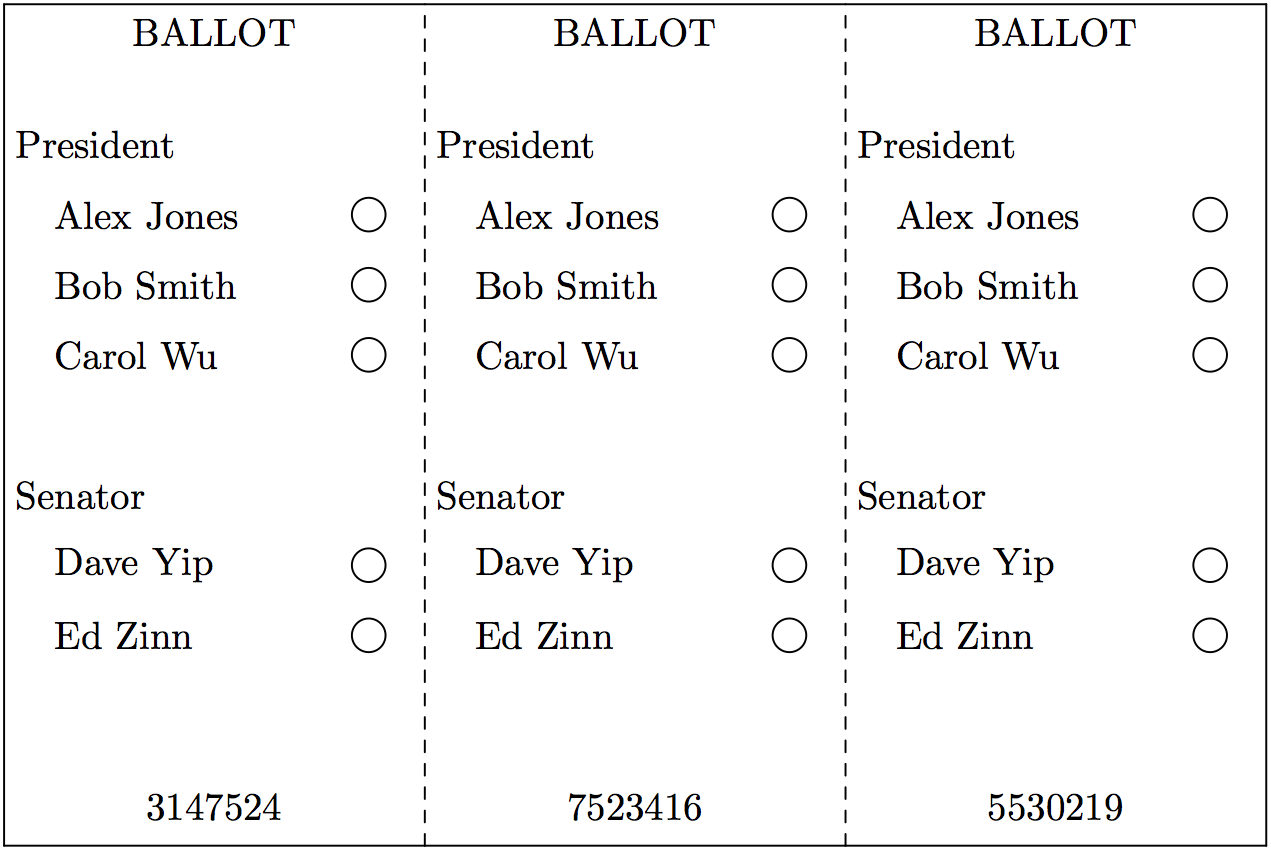
\includegraphics[width=0.5\linewidth]{ls/threeballot.png}
  \caption[Multi-Ballot]{Multi-Ballot~\cite{rivest_threeballot}}
  \label{fig:ls:threeballot}
\end{figure}

\npar Bij het invullen van het multi-ballot gelden de volgende regels. Elke rij van drie bolletjes komt overeen met \'e\'en kandidaat. Om voor een kandidaat te stemmen, moet de kiezer exact twee bolletjes inkleuren. Om tegen te stemmen, moet er \'e\'en bolletje aangeduid worden. In elke rij moeten exact \'e\'en of twee bolletjes ingevuld zijn, anders is het biljet ongeldig. Hoe de verschillende delen ingevuld zijn, maakt hierbij niet uit.

\npar Omdat het belangrijk is voor de telling dat de kiezer deze regels juist volgt, moet hij na het invullen van het biljet dit invoeren in een controlemachine. Wanneer het biljet niet correct ingevuld is, dan geeft de machine aan waar de kiezer een fout gemaakt heeft. Indien alles wel juist is aangeduid, dan wordt een rode streep geprint op het biljet waarna hij de aparte delen indient. Deze controlemachine mag geen enkele opname maken van de ingevoerde biljetten.

\npar Voordat hij de drie aparte biljetten afgeeft, moet de kiezer er willekeurig \'e\'en uitkiezen waarvan hij een kopie meekrijgt als ticket. Het is het veiligst om dit te implementeren in de controlemachine. Door de manier waarop het biljet ingevuld is, geeft het ticket geen informatie over hoe de kiezer gestemd heeft.

\subsubsection{Tellen van de stemmen}

Wanneer de verkiezing afgelopen is, worden alle biljetten gescand en de gegevens op het bulletin board gepost. Merk op dat het eigenlijke biljet niet online gezet wordt, omdat de kiezer hier iets op zou kunnen schrijven. Ook een lijst van iedereen die deelgenomen heeft aan de stemming, wordt ge\"upload. Een kiezer kan nu nagaan of zijn ticket ook op het bulletin board staat.

\npar Omdat alle stemmen op het bulletin board staan, kan iedereen zelf de telling verifi\"eren. De stemmen kunnen zoals anders geteld worden, zij het met een kleine aanpassing. Omdat er twee bolletjes gekleurd zijn bij een voorstem en maar \'e\'en bij een tegenstem, is het resultaat voor elke kandidaat vermeerderd met het aantal kiezers.

\subsubsection{Integriteit}
\label{sec:ls:integriteit}

Door het toevoegen van een ticket en het bulletin board kan de kiezer nagaan of zijn stembiljet gepubliceerd is en of het totale aantal geregistreerde biljetten klopt. Deze nieuwe controles zullen ons toelaten om verschillende vormen van fraude eenvoudig te detecteren. Het is ook belangrijk te kijken of zij zelf geen nieuwe zwakheden introduceren.

\npar Het toevoegen van nieuwe stemmen is onmogelijk zonder ook de lijst met kiezers aan te passen. Daarnaast kunnen er ook geen stemmen bijgewerkt of verwijderd worden zonder dat er mogelijk een kiezer komt klagen dat zijn stem niet correct online staat. Grootschalige fraude wordt op deze manier onmogelijk.

\npar Bij de \textit{Three-Pattern} aanval, vraagt de koper aan de kiezer om alle drie de delen in een bepaald patroon in te vullen. Wanneer hij dit patroon dan niet terugvindt op het bulletin board, wordt de kiezer niet betaald. Een mogelijke oplossing is het gebruik van een DRE machine. Deze print zelf de deelbiljetten in een willekeurig patroon, nadat de kiezer zijn keuze gemaakt heeft op een scherm.

\npar Bemerk tot slot dat de controlemachine die de geldigheid van de tickets nagaat zeer goed getest moet worden. Wanneer deze aangepast zou worden, kan ze bijvoorbeeld kiezers toelaten om voor een bepaalde kandidaat drie bolletjes te kleuren en voor een andere geen. Zo zouden die stemmen veel meer gewicht krijgen dan deze die zich wel aan de regels houden. Het is bovendien onmogelijk om dergelijke ongeldige patronen achteraf terug te vinden, omdat de verschillende biljetten los van elkaar worden ingediend.

\npar Tot slot zou een aanvaller kunnen betalen voor het ticket van de kiezer. Zo kan deze de correctheid van zijn stem niet meer nagaan. De aanvaller zou dan in theorie het biljet kunnen aanpassen dat op het bulletin board geplaatst werd. De kiezers moeten dus aangemoedigd worden om hun ticket niet af te geven. Deze aanval kan eenvoudig tegengegaan worden wanneer de kiezer zonder medeweten van de aanvaller een kopie maakt van het ticket. Voor een digitaal getekend ticket (bv. met een barcode) volstaat dit namelijk ook om klacht neer te leggen.

\subsubsection{Stemgeheim}

Zoals eerder aangehaald, bevat het ticket zelf geen informatie over hoe de kiezer gestemd heeft. Het mag echter ook niet mogelijk zijn om de drie deelbiljetten aan elkaar te linken. Het ID op het ticket zou anders gebruikt kunnen worden om uit te zoeken welk triplet van een bepaalde kiezer is. Een vereiste voor het systeem is ook dat niemand vooraf weet welke drie deelbiljetten zullen samenhoren. Een mogelijke oplossing hiervoor is om de delen apart te houden en er willekeurig drie te laten trekken door de kiezer.

\npar De kiezer mag zijn eigen multi-ballot niet kunnen reconstrueren op basis van de biljetten die op het bulletin board gepost worden. Dit kan opgelost worden door het ID te printen in de vorm van een 1D of 2D barcode, wat moeilijk te onthouden is. Het is ook verstandig om de kiezer geen vrije toegang te geven tot een kopieermachine bij het maken van het ticket. Dit is de reden waarom het ticket best geprint wordt door de controlemachine.

\npar Het moet ook onmogelijk zijn voor de kiezer om zijn stem nog te wijzigen nadat ze aanvaard is door de controlemachine. Een eerste oplossing is om hem geen fysische toegang meer te geven tot de biljetten nadat ze gecontroleerd zijn. Een tweede is om samen met de rode streep (\ref{sec:ls:multi-ballot}) een checksum op het biljet te printen die moeilijk veranderd kan worden door de kiezer.

\npar Tot slot moet er op gelet worden dat een reconstructie aanval niet mogelijk is. Hierbij haalt een aanvaller alle mogelijke geldige multi-ballots uit de biljetten die op het bulletin board geplaatst werden. Samen met het ticket van de kiezer, zou hij dan in sommige gevallen kunnen achterhalen hoe deze gestemd heeft. Om de integriteit van de stemming te kunnen controleren, heeft de kiezer alleen het ticket van een geldig biljet nodig. Het is dus niet noodzakelijk dat hij het ticket van zijn eigen biljet mee naar huis neemt. Een mogelijke manier om dit te implementeren is door gebruik te maken van floating receipts (\ref{sec:ls:floating_receipts}). Deze wordt niet expliciet vermeld in de paper van Rivest, maar hij bespreekt wel gelijkaardige methoden.\cite{rivest_threeballot}

\subsubsection{Bruikbaarheid}

Het ThreeBallot systeem is veel complexer dan de manier waarop nu gestemd wordt. De belangrijkste manier om ervoor te zorgen dat het systeem goed werkt, is dan ook het opleiden van de kiezer. Het is ook moeilijker om het biljet te corrigeren wanneer er een fout gemaakt wordt: meestal is de enige optie om opnieuw te beginnen met een blanco biljet. Het gebruik van een DRE machine zou het stemmen ook sterk vereenvoudigen. De kiezer moet dan wel controleren of het geprinte biljet correct is. In \ref{sec:ls:integriteit} werd reeds aangegeven dat dit ook de ThreePattern aanval onmogelijk maakt.

\npar Tot slot merken we nog op dat het tellen van de stemmen wel meer werk vraagt, aangezien er drie keer zoveel biljetten geteld moeten worden. ThreeBallot vergroot het vertrouwen van de kiezer in de integriteit van de verkiezing, ten koste van een moeilijker stemproces en meer werk bij het tellen.

\subsection{Scratch-Card}
\label{sec:ls:scratch_card}

Scratch-Card\cite{randell_ryan_voting_technologies_and_trust} maakt gebruik van een speciaal biljet dat makkelijk in twee gedeeld kan worden (\ref{fig:ls:scratch-card}). Belangrijk is dat de kandidaten op elk biljet in een willekeurige volgorde moeten staan. Een kiezer moet een willekeurig biljet trekken. Na het stemmen moet hij het linkerdeel vernietigen. Hij kan een kopie van het rechterdeel als ticket mee naar huis nemen.

\begin{figure}
  \centering
  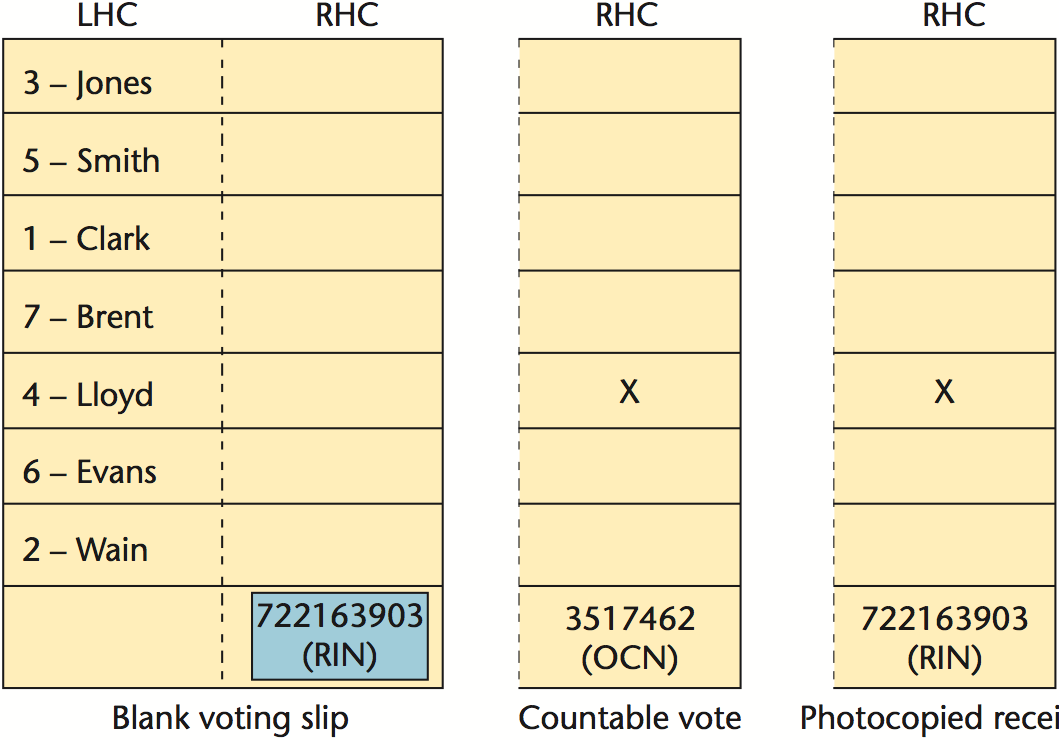
\includegraphics[width=0.5\linewidth]{ls/scratch-card.png}
  \caption[Scratch-Card biljet]{Scratch-Card biljet~\cite{randell_ryan_voting_technologies_and_trust}}
  \label{fig:ls:scratch-card}
\end{figure}

\npar Op het rechterdeel van het biljet is onderaan een kraslaag aangebracht. Bovenop deze laag is het unieke ID (RIN) van het biljet geprint dat de kiezer later kan gebruiken om zijn stem op het bulletin board terug te controleren. Bovendien verbergt deze laag een vooraf geprinte code die de volgorde van de kandidaten aangeeft (OCN). Bij het tellen wordt deze laag verwijderd en tegelijk verdwijnt ook het RIN van het biljet. Het is zeer belangrijk dat de RIN en OCN volledig ongecorreleerd zijn, want anders zou achterhaald kunnen worden van wie de stem is.

\npar Omdat het ticket een kopie is van het biljet met het kraslaagje nog intact, kan de OCN nooit meer achterhaald worden. Het is dus belangrijk goed te controleren dat de tellers niet proberen om RIN/OCN-combinaties neer te schrijven tijdens het verwijderen van het laagje.

\npar Een nadeel aan het voorgestelde systeem is dat iedereen die een origineel rechterdeel bemachtigt, kan achterhalen op wie dat biljet gestemd heeft. Er is gelukkig wel geen rechtstreekse link tussen de RIN en de persoon die gestemd heeft. Een alternatief systeem print daarom een ID op het linker- en rechterdeel (CIN). Op het rechterdeel zit deze CIN opnieuw onder een kraslaag. In deze variant moet de kiezer na het stemmen ook zijn linkerdeel in een doos deponeren. Als ticket krijgt hij weer een kopie mee van de rechterkant, waarop de kraslaag nog intact was.

\npar Om de stemmen te tellen, wordt opnieuw de kraslaag verwijderd zodat de CIN gelezen kan worden. Vervolgens moet de linkerkant met dezelfde CIN gevonden worden om te achterhalen op wie gestemd is. Het grootste probleem is dat het zoeken naar de juiste paren heel veel werk zou vragen bij grote verkiezingen, tenzij dit geautomatiseerd zou worden.

\npar Net zoals bij Twin (\ref{sec:ls:twin}) is het invullen van het biljet zeer eenvoudig voor de kiezer. Ook hier is het echter belangrijk dat de kiezers de juiste procedure volgen en een kopie nemen van hun biljet voordat de kraslaag verwijderd is. De bijzitters moeten dus toezien op het correct verloop van de verkiezing.

\section{Systemen met cryptografie}
\label{sec:ls:systemen_met_cryptografie}

De systemen in de vorige sectie maakten geen gebruik van ingewikkelde cryptografische technieken. Omdat het hierdoor eenvoudiger te begrijpen is, zal zo'n systeem sneller vertrouwd worden door de kiezer (\ref{sec:ls:vertrouwen}). In deze sectie worden toch enkele systemen besproken die hier wel op steunen. Door gebruik te maken van zero-knowledge bewijzen, homomorfe cryptografie en \textit{mixnets} kunnen immers veilige end-to-end verifiable systemen ontworpen worden.

\npar Bij Secret-Ballot Receipts (\ref{sec:ls:secret_ballot_receipts}) wordt optische cryptografie toegepast om de stem op het ticket te encrypteren. Scratch \& Vote (\ref{sec:ls:scratch_and_vote}) bouwt verder op de principes die geïntroduceerd werden bij Scratch-Card (\ref{sec:ls:scratch_card}).

\subsection[Secret-Ballot Receipts]{Secret-Ballot Receipts~\cite{chaum_secret_ballot}}
\label{sec:ls:secret_ballot_receipts}

Secret-Ballot Receipts werden in 2004 gepubliceerd door David Chaum. De kiezer ziet zijn stem geprint worden in het stemhokje en kan zijn ticket gebruiken om nadien te controleren of ze correct meegeteld is. Omdat zijn keuzes ge\"encrypteerd worden tijdens het printproces, kan hij het ticket niet gebruiken om te bewijzen hoe hij gestemd heeft. Bovendien is het niet nodig om vertrouwde hardware te gebruiken aangezien de publieke code op relatief eenvoudige systemen gedraaid kan worden.

\npar Nadat de kiezer zijn keuzes aangegeven heeft, worden deze door een speciale printer afgedrukt. De printer drukt tegelijk op beide kanten van het strookje afzonderlijke, maar uitgelijnde afbeeldingen. De kiezer wordt gevraagd om de afdruk te controleren en kan zijn stem eventueel nog aanpassen. Wanneer hij tevreden is, kan hij kiezen of hij de boven- of onderkant wil meenemen. Pas dan wordt het laatste stukje van het ticket afgedrukt en kan hij de twee delen uit de printer nemen, terwijl ze nog aan elkaar vastzitten.

\npar Door de twee kanten van elkaar los te maken, wordt de afbeelding op het strookje schijnbaar willekeurig. Het doorgelaten licht op de plaatsen waar geen van beide kanten bedrukt is, maakte de stem zichtbaar. Geen van beide lagen bevat dus informatie over hoe gestemd is. Het laatst geprinte stukje is verschillend omdat daar wel tekst opstaat die ook na het scheiden van de twee lagen nog gelezen kan worden. Op de ene kant wordt duidelijk aangegeven dat deze bijgehouden moet worden en op de andere dat hij afgegeven moet worden. Deze laatste wordt duidelijk zichtbaar voor de kiezer vernietigd.

\begin{figure}
  \centering
  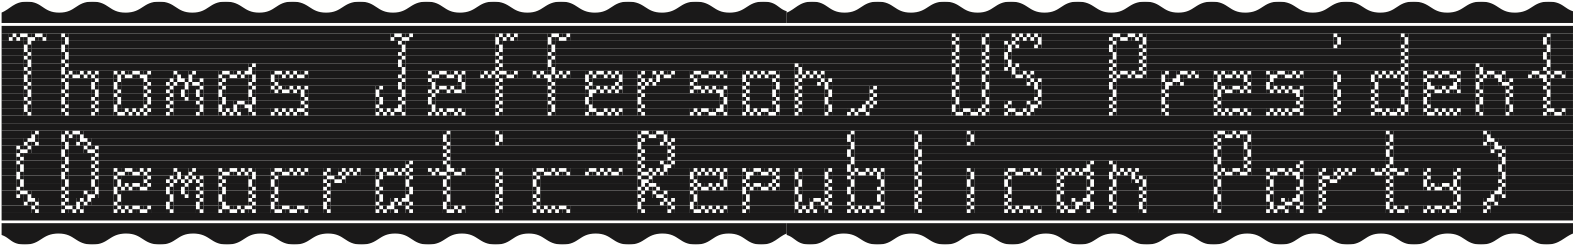
\includegraphics[width=0.5\linewidth]{ls/secret-ballot_vote.png}
  \caption[Strookje met optische ge\"encrypteerde stem]{Strookje met optische ge\"encrypteerde stem~\cite{chaum_secret_ballot}}
  \label{fig:ls:secret_ballot_vote}
\end{figure}

\begin{figure}
  \centering
  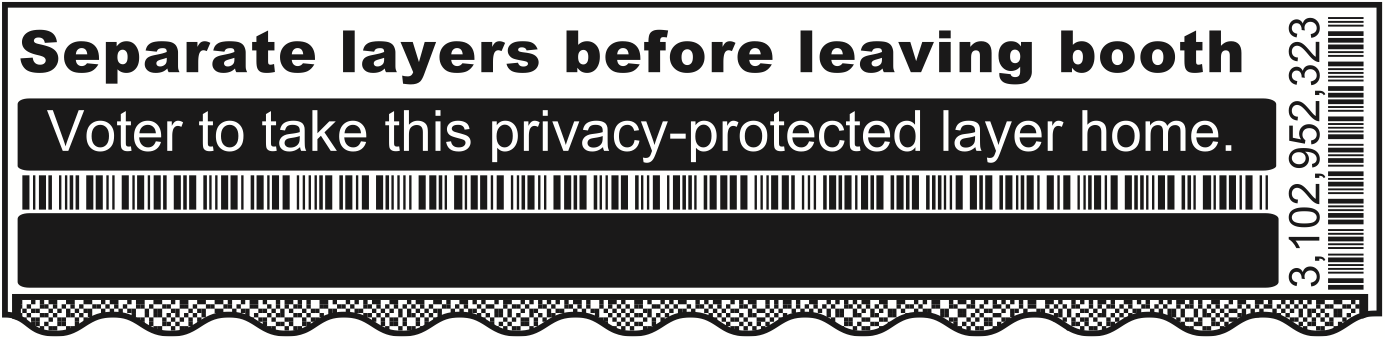
\includegraphics[width=0.5\linewidth]{ls/secret-ballot_receipt.png}
  \caption[Laatste stukje ticket met beide kanten nog samen]{Laatste stukje ticket met beide kanten nog samen~\cite{chaum_secret_ballot}}
  \label{fig:ls:secret_ballot_receipt}
\end{figure}

\npar De computer houdt zelf een digitale versie van het volledige ticket bij en verwijdert ook de data van de andere kant. Deze data wordt na het aflopen van de stemming ge\"upload naar een online bulletin board. Omdat het ticket geen informatie bevat over de stem van de kiezer, kan hij dit aan iedereen tonen zonder zijn stem openbaar te maken. Door het ticket te scannen kan eenvoudig vastgesteld worden of het authentiek is. Bij een ongeldige controle is men dus zeker dat de apparatuur niet correct gewerkt heeft.

\npar De kiezer kan na de stemming nagaan of zijn ticket juist op het bulletin board staat. Hij kan dit eenvoudig doen door te kijken of de versie die daar staat volledig overeenkomt met zijn eigen ticket. Na het afsluiten van de stemming wordt de uiteindelijke verzameling van stemmen die geteld moeten worden, online gezet. Er worden ook digitale handtekeningen van de set gepubliceerd die gebruikt kunnen worden om de echtheid ervan te controleren. Wanneer de stemmen geteld zijn, wordt een nieuwe set online geplaatst. Deze bevat evenveel biljetten, maar nu zijn de afbeeldingen gedecrypteerd en is elke stem leesbaar. Om de privacy van de kiezer te bewaren, zijn de biljetten willekeurig geordend.

\npar Er wordt gebruik gemaakt van een audit proces om te controleren of beide sets identiek dezelfde biljetten bevatten. Het telproces verloopt in verschillende stappen en na elke stap wordt een klein aantal willekeurig gekozen biljetten van de set gedecrypteerd tussen twee stappen in het telproces. Deze biljetten worden zo gekozen dat ze onvoldoende informatie bevatten om een kiezer te identificeren, maar wel gebruikt kunnen worden om na te gaan of er geen biljetten toegevoegd, verwijderd of gewijzigd werden.

\npar Omdat de optische encryptie neerkomt op een \textit{one-time path}, kan zelfs een aanvaller met ongelimiteerde rekenkracht de stem niet achterhalen. De gebruikte sleutels zijn dus de pixels van één van beide kanten. Deze zijn niet willekeurig, maar in de praktijk kunnen ze hiervan niet onderscheiden worden, tenzij door de personen die de decryptie zullen uitvoeren.

\npar Aangezien alles digitaal opgeslagen wordt, kan de telling ook voor grote verkiezingen effici\"ent uitgevoerd worden. Een bijkomend voordeel is dat kiezers via een computer moeten stemmen, wat ze vaak reeds gewoon zijn. Hoewel de software op eenvoudige machines kan draaien, zijn er nog steeds speciale printers nodig om de tickets af te drukken. 

\subsection[Scratch \& Vote]{Scratch \& Vote~\cite{adida_rivest_scratch_and_vote}}
\label{sec:ls:scratch_and_vote}

Scratch \& Vote werd in 2006 ontworpen door Ben Adida en Ronald L. Rivest. Het is een variatie op Scratch-Card (\ref{sec:ls:scratch_card}) waarbij gebruik gemaakt wordt van homomorfe cryptografie en zero-knowledge correctheidsbewijzen. Iedereen kan het uiteindelijke resultaat verifi\"eren en alleen de cijfertekst van de uitslag moet gedecrypteerd worden door de verantwoordelijken van de verkiezing. Het grote verschil met Scratch-Card (\ref{sec:ls:scratch_card}) is dat er niet langer met een RIN/CIN gewerkt moet worden, net omdat de stemmen nu ge\"encrypteerd worden.

\npar Bij het aanmelden ontvangt de kiezer een biljet dat uit twee delen bestaat. Op de linkerzijde staan de kandidaten in een willekeurige volgorde, die alleen door de kiezer gezien mag worden. Op de rechterkant kan de kiezer zijn stem uitbrengen. Onderaan dit deel staan verder een 2D barcode en een kraslaag. Net zoals bij Scratch-Card wordt de linkerkant na het invullen van het biljet in het stemhokje afgescheurd en in een doos gedeponeerd. Een bijzitter controleert of de kraslaag op de rechterkant nog intact is en verwijdert deze daarna. Vervolgens wordt dit stukje zichtbaar voor de kiezer vernietigd. Tot slot laat de kiezer de eigenlijke stem en barcode scannen. Wanneer het stukje met de kraslaag verwijderd is van het biljet, bevat het rechterdeel geen informatie meer die gebruikt kan worden om de stem van de kiezer te achterhalen. Het gescande deel kan dus als ticket meegenomen worden.

\npar Door aan te melden op het bulletin board, kan de kiezer controleren of zijn biljet correct gescand werd. Omdat alle gescande biljetten online geplaatst worden, kan iedereen nagaan of de cijfertekst van de eindtelling correct is.

\begin{figure}
  \centering
  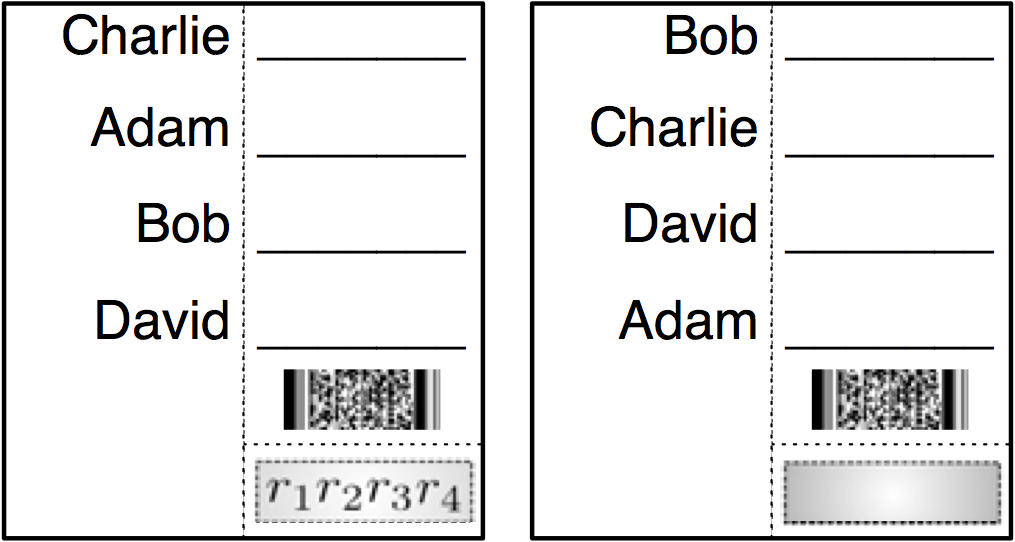
\includegraphics[width=0.5\linewidth]{ls/scratch_and_vote_ballot.png}
  \caption[Scratch \& Vote biljet]{Scratch \& Vote biljet~\cite{adida_rivest_scratch_and_vote}}
  \label{fig:ls:scratch_and_vote_ballot}
\end{figure}

\npar Voor de encryptie wordt gebruik gemaakt van het Paillier public key cryptosystem. Dit systeem heeft een additief homomorfisme door het vermenigvuldigen van de cijferteksten. Het tellen van de stemmen bij een verkiezing met meerdere kandidaten zou echter niet mogelijk zijn zonder gebruik te maken van een \textit{multi-counter}. Het aantal beschikbare bits voor de leesbare tekst wordt onderverdeeld in verschillende tellers. Hierbij worden voldoende bits beschikbaar gemaakt voor elke teller zodat ze niet in elkaar kunnen overlopen.

\npar Het systeem maakt daarnaast gebruik van zero-knowledge bewijzen. Deze worden gebruikt om aan te tonen dat een set cijferteksten $c_1, c_2, \ldots, c_l$ de encryptie is van de permutatie van $m_1, m_2, \ldots, m_k$ (ervan uitgaande dat geen twee subsets van ${m_i}$ dezelfde som hebben). De verschillende ${m_i}$ zijn de tellers voor de kandidaten.

\npar Daarnaast worden ook bewijzen opgesteld die aantonen dat de biljetten zelf correct zijn. Omdat deze bewijzen te lang zijn om op de biljetten te printen, worden ze voor de start van de verkiezing ge\"upload naar het bulletin board. Ze worden tijdens het tellen van de stemmen gebruikt om te verzekeren dat elk biljet maar \'e\'en stem uitbrengt per verkiezing. Om de kiezer te garanderen dat zijn biljet tijdens het tellen niet ongeldig verklaard zal worden, wordt ook een offici\"ele lijst van alle geldige biljetten voorzien. De kiezer kan dan eenvoudig nagaan of zijn biljet hierop voorkomt.

\begin{figure}
  \centering
  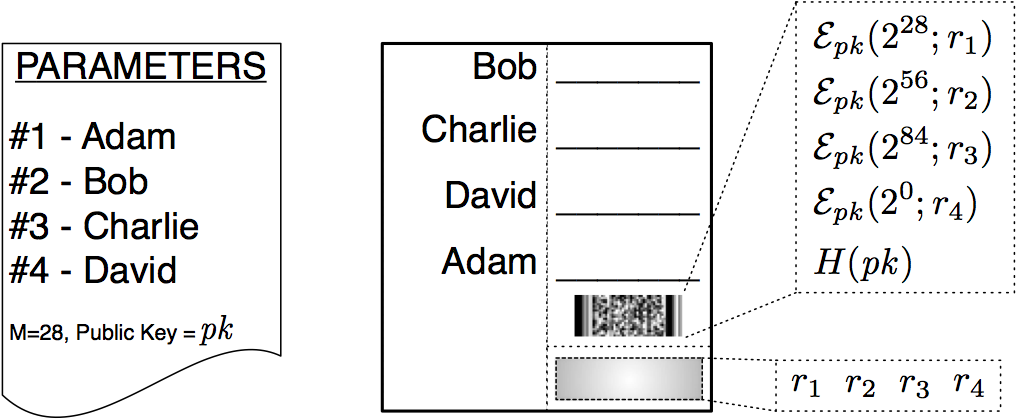
\includegraphics[width=0.5\linewidth]{ls/scratch_and_vote_encryption.png}
  \caption[Scratch \& Vote encryptie]{Scratch \& Vote encryptie~\cite{adida_rivest_scratch_and_vote}}
  \label{fig:ls:scratch_and_vote_encryption}
\end{figure}

\npar De 2D barcode op elk biljet encodeert de willekeurige volgorde van de cijferteksten voor de verschillende kandidaten samen met een hash van de publieke sleutel (\ref{fig:ls:scratch_and_vote_encryption}). De startwaarde van de teller van elke kandidaat wordt samen met een willekeurige waarde ge\"encrypteerd. Zo heeft ieder biljet een unieke cijfertekst voor elke kandidaat. Deze willekeurige waarden worden verborgen door de kraslaag. De startwaarden van de tellers vormen met de publieke sleutel de gepubliceerde parameters. Samen met de willekeurige waarden kunnen ze dus gebruikt worden om de volgorde van de kandidaten op het biljet te achterhalen. Daarom is het belangrijk dat dit stukje van het biljet vernietigd wordt.

\npar Deze informatie wordt toch op de biljetten geprint omdat ze nodig is voor een audit. Dit wordt gedaan door de kiezer twee biljetten te laten kiezen. Door de kraslaag weg te halen, worden de willekeurige waarden zichtbaar en kan nagegaan worden of het biljet correct is. Door het verwijderen van de kraslaag wordt het biljet ongeldig, wat de reden is dat de kiezer twee biljetten moet nemen. Op deze manier wordt de helft van de biljetten getest en dus is de kans groot dat foutieve biljetten gedetecteerd worden.

\npar Zowel naar de kiezer als de bijzitters toe is dit systeem zeer gebruiksvriendelijk. Het standaard stembiljet is slechts licht gewijzigd en de kiezer zou er dus vertrouwd mee moeten zijn. Ook de stemprocedure is niet radicaal gewijzigd. Aangezien de telprocedure ook geautomatiseerd is, kan deze methode ook voor grote verkiezingen gebruikt worden.

\section[Online stemmen]{Online stemmen~\cite{adida_helios}}
\label{sec:ls:online_stemmen}

Een mogelijkheid om mensen van op afstand te laten stemmen, is door een online verkiezingssysteem te gebruiken. Studies hebben aangetoond dat technologie\"en die het eenvoudiger maken om te stemmen de opkomst kunnen verbeteren.\cite{news:guardian_shaking_up_voter_apathy_with_it} Het voornaamste probleem bij dit soort systemen is dat de omgeving niet langer gecontroleerd kan worden door de organisator van de verkiezing. Bij een online verkiezing kan de kiezer gedwongen worden om op een bepaalde manier te stemmen, terwijl de aanvaller over zijn schouder meekijkt. Het is voor de kiezer ook eenvoudiger zijn stem te verkopen aangezien hij op dezelfde manier kan bewijzen aan de koper dat hij correct gestemd heeft.

\npar Helios lost dit probleem niet op, maar stelt dat er situaties zijn waar het gevaar op een aanval kleiner is omdat de inzet er minder groot is. Voorbeelden zijn verkiezingen bij een lokale sportclub of studentenorganisaties. Hier is echter wel nog steeds nood aan een betrouwbaar en geheim verkiezingssysteem. Een online verkiezingssysteem is hier dan ook ideaal, omdat de organisatie van de verkiezing anders veel meer werk zou vragen.

\section{Conclusie}
\label{sec:ls:conclusie}

Bij open counting (\ref{sec:ls:open_counting}) wordt een transparante manier van tellen gebruikt om het vertrouwen van de kiezer in het resultaat te vergroten. In tegenstelling tot de andere systemen kan door de kiezer wel niet nagegaan worden of zijn stem meegeteld is. Voter-verifiability wordt daar bekomen door gebruik te maken van een ander type biljet samen met een aangepaste stemprocedure.

\npar Deze aanpassingen maken het stemmen voor de kiezer ingewikkelder. In tegenstelling tot bij een klassiek biljet, moeten nu verschillende regels gevolgd worden om het biljet correct in te vullen. De stemprocedures zijn vaak ook ingewikkelder dan voordien, met nieuwe regels voor zowel de kiezers als de bijzitters.

\npar Door cryptografische technieken te gebruiken, kan de gebruiksvriendelijkheid van papieren end-to-end verifiable systemen sterk verbeterd worden. Een nadeel is hier dan weer dat de meeste mensen nog steeds zullen moeten vertrouwen op het oordeel van een expert over de correctheid van het systeem.

\npar Papieren voter-verifiable systemen hebben dus enkele grote nadelen die hun praktisch nut sterk beperken. Ze zijn vaak zeer complex en niet bruikbaar voor grote verkiezingen. Cryptografische technieken lossen deze problemen wel deels op, maar worden dan weer moeilijker vertrouwd door de kiezer.

\npar Helios is in de eerste plaats een systeem dat toelaat om online verkiezingen te organiseren. Deze systemen kunnen echter alleen gebruikt worden wanneer het gevaar op dwang klein is. Het is hier immers niet mogelijk om de omgeving waarin de kiezer zijn stem uitbrengt te controleren, waardoor het voor een aanvaller eenvoudiger is om invloed uit te oefenen.
